\documentclass[border=1mm]{standalone}

\usepackage{listings}
\usepackage{tikz}
\usetikzlibrary{positioning,fit,calc}
\usetikzlibrary{shapes.multipart}
\pgfsetlayers{background,cpu,main}

\pgfdeclarelayer{background}
\pgfdeclarelayer{cpu}
\pgfdeclarelayer{main}

\newsavebox\mybox

\lstset{language=Python}


\begin{document}

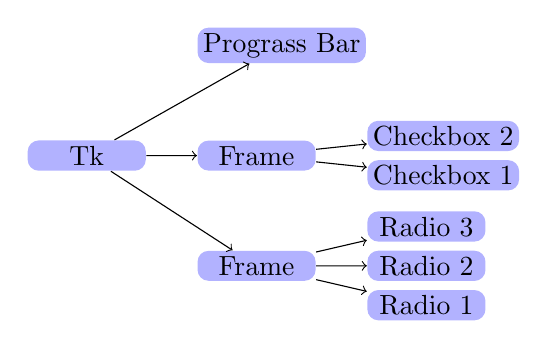
\begin{tikzpicture}[
        level/.style={sibling distance = 10mm,
                      level distance = 14mm},
        level 1/.style={sibling distance = 14mm},
        level 2/.style={sibling distance = 5mm}]
  \tikzstyle{every node}=[text centered,rounded corners, fill=blue!30,
    minimum width=15mm,grow=right,inner sep=2pt]
  \tikzstyle{every path}=[->]
     \node {Tk} [grow=0,right]
       child {
         node {Frame}
         child { node {Radio 1}}
         child { node {Radio 2}}
         child { node {Radio 3}}
      }
      child {
         node {Frame}
         child { node {Checkbox 1} }
         child { node {Checkbox 2}}
       } 
       child { node {Prograss Bar} }
    ;
\end{tikzpicture}

\end{document}

